%% supplement.tex -- supplementary material for the paper (same class/styles).
%% Build: make -C doc -f doc.mk supplement  (requires a prior full paper build
%% so that build/main.aux provides the paper's section/figure numbers).
\documentclass[conference]{IEEEtran}
\IEEEoverridecommandlockouts
% preamble.tex — master preamble for the CGRA report.
%
% This file only *orchestrates* the modular configuration; each concern lives
% in its own file so it can be read, reused or replaced in isolation. The load
% order is significant:
%
%   1. package    — every \usepackage except hyperref
%   2. colors     — palette (needs xcolor)
%   3. tikz       — libraries + node/edge styles (needs tikz + colors)
%   4. macros     — document-level helper commands
%   5. hyperref   — links, metadata, PDF bookmarks (MUST be loaded last)

% package.tex — package declarations for the CGRA report.
%
% Loaded first by config/preamble.tex and kept deliberately free of any
% configuration (colours, styles, macros and hyperref live in their own
% modules) so the dependency list stays readable at a glance.
%
% Ordering note: hyperref must be the *last* package loaded, after cite and
% url, so it is pulled in separately by config/hyperref.tex — do not add it
% here.

% ---- encoding & fonts ----------------------------------------------------
\usepackage[T1]{fontenc}      % 8-bit output encoding, hyphenatable accents
\usepackage[utf8]{inputenc}   % UTF-8 source
\usepackage{microtype}        % character protrusion / font expansion
\usepackage{mathptmx}         % Times math, matching IEEEtran's Times text
\usepackage{tgheros}          % TeX Gyre Heros: sans for figures/labels
\renewcommand{\ttdefault}{txtt} % legible monospace for literals and bytes

% ---- mathematics ---------------------------------------------------------
\usepackage{amsmath}
\usepackage{amssymb}

% ---- tables --------------------------------------------------------------
\usepackage{booktabs}         % \toprule \midrule \bottomrule
\usepackage{array}            % extended column types, \newcolumntype
\usepackage{tabularx}         % full-width tables with wrapping columns
\usepackage{colortbl}         % light header shading in tables

% ---- graphics & diagrams -------------------------------------------------
\usepackage{graphicx}
\usepackage{xcolor}
\usepackage{tikz}
\usepackage{pgfplots}         % measured-data plots (figures/cost/diagram.tex)
\pgfplotsset{compat=1.18}

% ---- bibliography & URLs -------------------------------------------------
\usepackage{cite}             % compressed, sorted numeric citations
\usepackage{url}

% colors.tex — one restrained, print-safe palette for figures, tables and
% links. Requires xcolor (see config/package.tex); loaded before tikz/hyperref.
%
% Each role has a light fill and a dark edge of the same hue. The four hues
% (slate blue, ochre, teal, plum) remain distinguishable in greyscale by
% lightness and in the common colour-vision deficiencies by hue+lightness;
% figures never rely on colour alone (labels/shapes carry the meaning).

% ---- figure roles (block / ALU / register / state / wire) ----------------
\definecolor{cBlock}{HTML}{E9EEF5}   % logic blocks, PEs, muxes
\definecolor{cBlockE}{HTML}{2F5A8A}
\definecolor{cAlu}{HTML}{F6EBD8}     % arithmetic
\definecolor{cAluE}{HTML}{A3741E}
\definecolor{cReg}{HTML}{E2F0EC}     % registers / storage
\definecolor{cRegE}{HTML}{2E7D6B}
\definecolor{cState}{HTML}{F0E8F2}   % FSM states
\definecolor{cStateE}{HTML}{7A4A84}
\definecolor{cWire}{HTML}{3A3F47}    % wires, axes, annotations

% ---- evidence status (figures/evidence, tables) ---------------------------
\definecolor{cPass}{HTML}{2E7D6B}    % executed and passed
\definecolor{cPart}{HTML}{A3741E}    % bounded / partial / conditional
\definecolor{cNone}{HTML}{9AA1AB}    % not run
\definecolor{cHead}{HTML}{EEF1F5}    % table header shading

% ---- hyperlinks (config/hyperref.tex) -------------------------------------
% One dark accent for every link kind: legible in print, visible on screen.
\definecolor{cLink}{HTML}{1F4E79}
\definecolor{cCite}{HTML}{1F4E79}

% tikz.tex — TikZ libraries and the reusable node/edge styles shared by every
% figure in figures/*.tex. Requires tikz and the colour palette (config/colors).

\usetikzlibrary{
  arrows.meta,
  automata,
  positioning,
  calc,
  fit,
  backgrounds,
  shapes.geometric,
  shapes.misc,
  matrix,
  decorations.pathreplacing
}

% Figures use the sans family (TeX Gyre Heros) for labels, as is customary
% in IEEE figures; mathematics keeps the text math font. Node styles below set
% only the size, so the family set here is inherited everywhere.
\tikzset{
  every picture/.append style={/utils/exec={\sffamily}},
  blk/.style   ={draw=cBlockE, fill=cBlock, rounded corners=2pt,
                 minimum height=8mm, minimum width=16mm, align=center,
                 font=\small},
  alu/.style   ={draw=cAluE, fill=cAlu, trapezium, trapezium angle=68,
                 shape border rotate=270, minimum width=12mm,
                 minimum height=9mm, align=center, font=\small},
  reg/.style   ={draw=cRegE, fill=cReg, rounded corners=1pt,
                 minimum height=7mm, minimum width=10mm, align=center,
                 font=\small},
  mux/.style   ={draw=cBlockE, fill=cBlock, trapezium, trapezium angle=70,
                 shape border rotate=90, minimum width=10mm,
                 minimum height=7mm, align=center, font=\footnotesize},
  pe/.style    ={draw=cBlockE, fill=cBlock, rounded corners=2pt,
                 minimum size=11mm, align=center, font=\footnotesize},
  st/.style    ={draw=cStateE, fill=cState, circle, minimum size=10mm,
                 align=center, font=\scriptsize, inner sep=1pt},
  wire/.style  ={-{Latex[length=2mm]}, color=cWire, thick},
  wireb/.style ={{Latex[length=2mm]}-{Latex[length=2mm]}, color=cWire, thick},
  lbl/.style   ={font=\scriptsize, color=cWire}
}

% macros.tex — small helper macros used across the report body.

\newcommand{\cmd}[1]{\texttt{#1}}          % protocol command / literal token
\newcommand{\reg}[1]{\ensuremath{\mathrm{#1}}} % a register / scalar symbol
\newcommand{\byte}[1]{\texttt{0x#1}}       % a literal byte value

% Array geometry as symbols, so the prose tracks hw/rtl/cgra_pkg.vhd.
\newcommand{\Rows}{\ensuremath{R}}
\newcommand{\Cols}{\ensuremath{C}}

% Table header row: light shading, bold sans labels (use after \toprule).
\newcommand{\thead}[1]{\textsf{\bfseries #1}}
\newcommand{\headrow}{\rowcolor{cHead}}

% Evidence-status marks, also explained in the caption of Fig. evidence.
\newcommand{\stpass}{\tikz[baseline=-0.6ex]\fill[cPass] (0,0) circle (0.9ex);}
\newcommand{\stpart}{\tikz[baseline=-0.6ex]{\fill[cPart] (0,0) -- (90:0.9ex)
  arc (90:270:0.9ex) -- cycle; \draw[cPart, line width=0.5pt] (0,0) circle (0.85ex);}}
\newcommand{\stnone}{\tikz[baseline=-0.6ex]\draw[cNone, line width=0.7pt] (0,0) circle (0.8ex);}
\newcommand{\stna}{\textcolor{cNone}{--}}

% Rules that touch the shaded header row without booktabs' white padding:
%   \headtop \headrow \thead{..} & ... \\ \headbottom
\newcommand{\headtop}{\specialrule{\heavyrulewidth}{0pt}{0pt}}
\newcommand{\headbottom}{\specialrule{\lightrulewidth}{0pt}{2pt}}

% Numbers derived from archived data (generated by doc.mk before LaTeX runs):
% tools/model_data.py and tools/scaling_data.py. Never type these by hand.
\input{build/model-macros}
\input{build/scaling-macros}

% Implementation values transcribed from archived run manifests (see file).
% Routed run at 5.859 ns on the current revision, executed for this paper.
% Source: doc/review/evidence/vivado-sta5859-20261015/manifest.json
% (run sta-20261015T152452Z-c35ee8fc; values checked against timing_summary).
\newcommand{\VivadoFastWNS}{$+0.177$}
\newcommand{\VivadoFastWHS}{$+0.122$}
\newcommand{\VivadoFastLUT}{4\,999/4\,975}
\newcommand{\VivadoFastFF}{1\,034}
\newcommand{\VivadoFastSummary}{WNS $+0.177$\,ns, WHS $+0.122$\,ns, identical to the archived candidate}

\input{build/ana-macros}

% hyperref.tex — PDF hyperlinks, document metadata and the viewer-side
% bookmark tree (the navigable "table of contents" pane a PDF reader shows
% next to the page). Loaded LAST by config/preamble.tex, after cite and url,
% as hyperref requires; the colours come from config/colors.tex.

\usepackage[
  bookmarks=true,
  bookmarksopen=true,
  bookmarksopenlevel=2,
  bookmarksnumbered=true,
  colorlinks=true,
  linkcolor=cLink,
  citecolor=cCite,
  urlcolor=cLink,
  pdfstartview=FitH,
  pdfpagemode=UseOutlines,   % open with the bookmark pane visible
  pdfdisplaydoctitle=true
]{hyperref}
\usepackage{bookmark}        % single-pass, reorderable bookmarks

\hypersetup{
  pdftitle    = {Communication Costs and Verification of a Step-Controlled FPGA CGRA},
  pdfauthor   = {Mattia Fait},
  pdfsubject  = {Host--accelerator communication and verification of a CGRA on FPGA},
  pdfkeywords = {CGRA, FPGA, host-accelerator communication, performance modelling, formal verification, multicycle constraints}
}


\usepackage{xr-hyper}
\externaldocument[P-]{build/main}
\graphicspath{{figures/}}
\renewcommand{\thesection}{S\arabic{section}}
\renewcommand{\thefigure}{S\arabic{figure}}
\renewcommand{\thetable}{S\Roman{table}}

\begin{document}
\title{Supplementary Material:\\Communication Costs and Verification of a\\
Step-Controlled FPGA CGRA}
\author{\IEEEauthorblockN{Mattia Fait}\IEEEauthorblockA{University of Trento\\Trento, Italy}}
\maketitle

\begin{abstract}
This supplement collects material that supports the paper but is not needed
to follow its argument: controller and wire-level details, the host software
stack, an illustration of capture spacing, alternative presentations of
data already tabulated in the paper, the planned board-acceptance procedure
with its (empty) report figure, and the chronology of the formal and
implementation runs, including failed attempts. References of the form
``Section~P-x'' point to the paper.
\end{abstract}

\section{Controller and wire-level details}

\subsection{Controller state machine}
Fig.~\ref{fig:fsm} shows the controller of \texttt{cgra\_ctrl} with the RTL
state names. From \texttt{S\_IDLE} the first received byte selects a branch.
Short transactions (\cmd{ID}, \cmd{RST} and the rejection of an unknown
opcode) reply at once through the shared transmit handshake. Bulk transfers
accumulate their payload, receive and verify the checksum in a dedicated
state and reply \cmd{ACK} or \cmd{NACK}. \cmd{RUN} produces $N$ enabled PE
captures at the configured cadence before acknowledging. The \cmd{EXEC}
header state falls through into the same receive state as \cmd{WR} and the
same step engine as \cmd{RUN}; only the return targets, held in two
registers, differ. A watchdog guards every state that waits for a payload
or checksum byte. After an uncertain transfer the library clears its cached
identity and fails later calls with \texttt{CGRA\_ERR\_DESYNC}; it sends no
implicit \cmd{RST}, because a controller waiting for a \cmd{RUN} argument
would interpret that byte (\byte{06}) as a step count.

\begin{figure*}[t]
  \centering
  \resizebox{\textwidth}{!}{% Controller state machine (hw/rtl/cgra_ctrl.vhd). Each box is one RTL state
% or a short chain of them (named in typewriter); byte loops and the shared
% transmit handshake S_SEND/S_SEND_WAIT are folded into the boxes that use it.
% Blue boxes are the states shared by two commands: S_WR (WR, EXEC) and
% S_RUN (RUN, EXEC); the return target is held in wr_ret / run_ret.
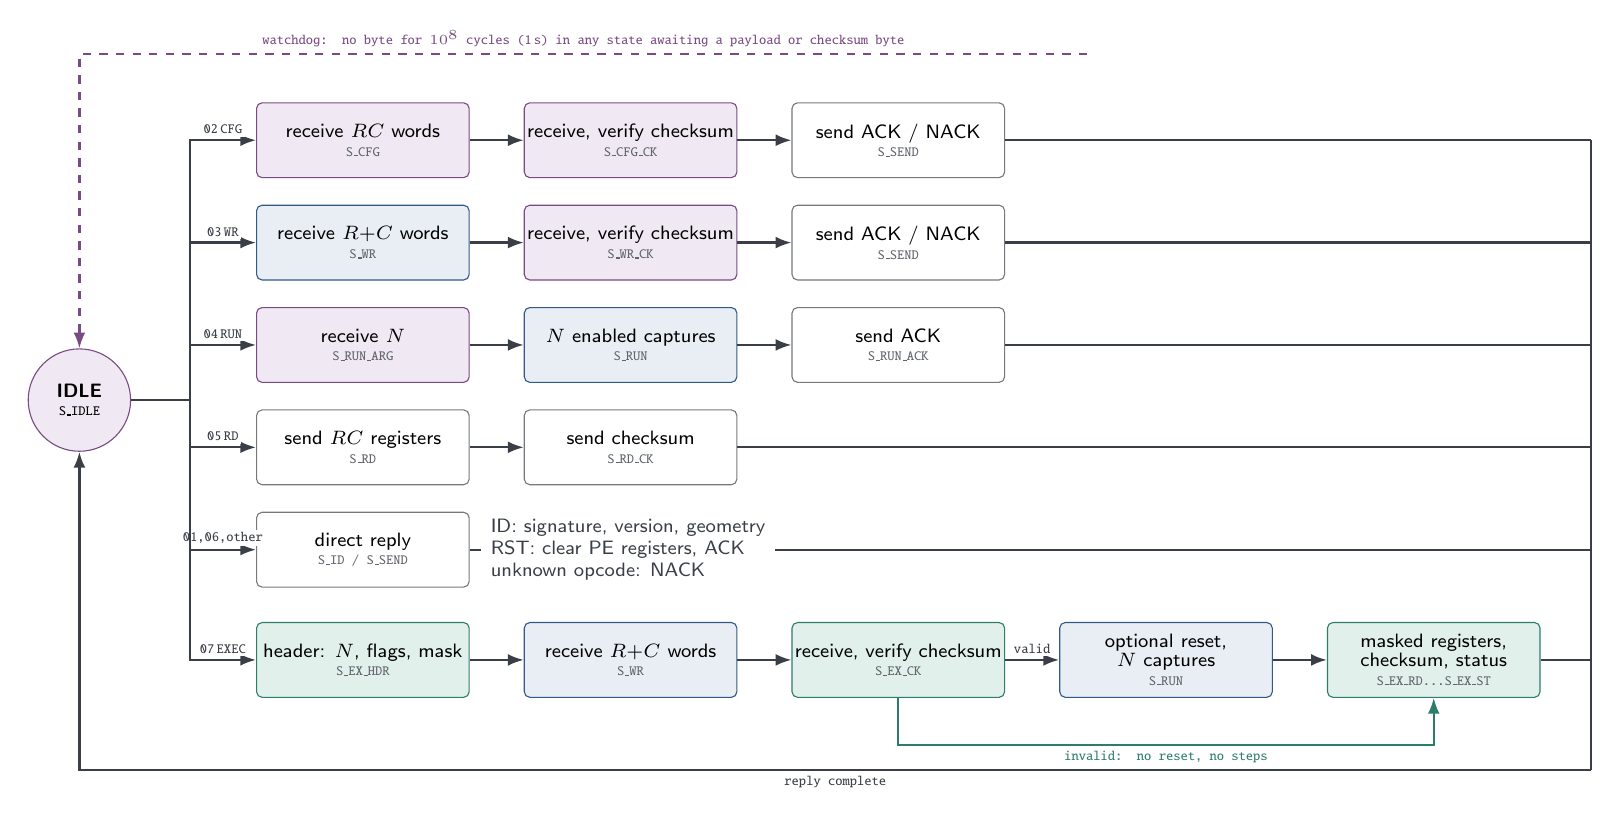
\begin{tikzpicture}[x=1mm, y=1mm, font=\scriptsize,
    st/.style={draw=cStateE, fill=cState, rounded corners=2pt,
      minimum width=27mm, minimum height=9.5mm, align=center, inner sep=1pt},
    sh/.style={st, draw=cBlockE, fill=cBlock},
    ex/.style={st, draw=cRegE, fill=cReg},
    tx/.style={st, draw=cWire!70, fill=white},
    sn/.style={font=\tiny\ttfamily, text=cWire!80},
    op/.style={lbl, fill=white, inner sep=1pt, font=\tiny\ttfamily}]
  \newcommand{\stbox}[5]{\node[#1] (#2) at #3 {#4\\[-0.4ex]{\tiny\ttfamily\color{cWire!80}#5}};}

  % hub
  \node[draw=cStateE, fill=cState, circle, minimum size=13mm, align=center,
        font=\scriptsize\bfseries] (idle) at (0,0) {IDLE\\[-0.5ex]{\tiny\ttfamily\mdseries S\_IDLE}};

  % one row per command family: y positions
  \def\yCFG{33} \def\yWR{20} \def\yRUN{7} \def\yRD{-6} \def\yID{-19} \def\yEX{-33}

  \stbox{st}{cfg1}{(36,\yCFG)}{receive $RC$ words}{S\_CFG}
  \stbox{st}{cfg2}{(70,\yCFG)}{receive, verify checksum}{S\_CFG\_CK}
  \stbox{tx}{cfg3}{(104,\yCFG)}{send ACK / NACK}{S\_SEND}

  \stbox{sh}{wr1}{(36,\yWR)}{receive $R{+}C$ words}{S\_WR}
  \stbox{st}{wr2}{(70,\yWR)}{receive, verify checksum}{S\_WR\_CK}
  \stbox{tx}{wr3}{(104,\yWR)}{send ACK / NACK}{S\_SEND}

  \stbox{st}{run1}{(36,\yRUN)}{receive $N$}{S\_RUN\_ARG}
  \stbox{sh}{run2}{(70,\yRUN)}{$N$ enabled captures}{S\_RUN}
  \stbox{tx}{run3}{(104,\yRUN)}{send ACK}{S\_RUN\_ACK}

  \stbox{tx}{rd1}{(36,\yRD)}{send $RC$ registers}{S\_RD}
  \stbox{tx}{rd2}{(70,\yRD)}{send checksum}{S\_RD\_CK}

  \stbox{tx}{id1}{(36,\yID)}{direct reply}{S\_ID / S\_SEND}
  \node[lbl, align=left, anchor=west] (idl) at (51,\yID)
    {ID: signature, version, geometry\\RST: clear PE registers, ACK\\unknown opcode: NACK};

  \stbox{ex}{ex1}{(36,\yEX)}{header: $N$, flags, mask}{S\_EX\_HDR}
  \stbox{sh}{ex2}{(70,\yEX)}{receive $R{+}C$ words}{S\_WR}
  \stbox{ex}{ex3}{(104,\yEX)}{receive, verify checksum}{S\_EX\_CK}
  \stbox{sh}{ex4}{(138,\yEX)}{optional reset,\\[-0.4ex] $N$ captures}{S\_RUN}
  \stbox{ex}{ex5}{(172,\yEX)}{masked registers,\\[-0.4ex] checksum, status}{S\_EX\_RD\dots S\_EX\_ST}

  % dispatch from IDLE: orthogonal fan-out with opcode labels
  \foreach \y/\dst/\code in {\yCFG/cfg1/02\,CFG, \yWR/wr1/03\,WR, \yRUN/run1/04\,RUN,
                             \yRD/rd1/05\,RD, \yID/id1/{01,06,other}, \yEX/ex1/07\,EXEC} {
    \draw[wire] (idle.east) -| (14,\y) -- node[op, above=0.3mm] {\code} (\dst.west);
  }

  % forward edges
  \foreach \a/\b in {cfg1/cfg2, cfg2/cfg3, wr1/wr2, wr2/wr3, run1/run2, run2/run3,
                     rd1/rd2, ex1/ex2, ex2/ex3} \draw[wire] (\a) -- (\b);
  \draw[wire] (ex3) -- node[op, above=0.3mm] {valid} (ex4);
  \draw[wire] (ex4) -- (ex5);
  \draw[wire, cRegE] (ex3.south) -- ++(0,-6) -| node[op, pos=0.25, below=0.3mm, text=cRegE]
    {invalid: no reset, no steps} (ex5.south);

  % return to IDLE through one bus on the right and below
  \def\xb{192}
  \foreach \n in {cfg3, wr3, run3, rd2, idl, ex5} \draw[cWire, thick] (\n.east) -- (\xb, |- \n.east);
  \draw[cWire, thick] (\xb,\yCFG) -- (\xb,-47);
  \draw[wire] (\xb,-47) -- node[op, below=0.3mm] {reply complete} (0,-47) -- (idle.south);
  \draw[cWire, thick] (id1.east) -- (idl.west);

  % watchdog (dashed): from every receive state back to IDLE
  \draw[wire, dashed, cStateE] (128,44) -- node[op, above=0.3mm, text=cStateE]
    {watchdog: no byte for $10^{8}$ cycles (1\,s) in any state awaiting a payload or checksum byte}
    (0,44) -- (idle.north);
\end{tikzpicture}
}
  \caption{Controller state machine of \texttt{cgra\_ctrl}. Boxes give the
  function and the RTL state(s) in typewriter; byte loops and the shared
  transmit handshake are folded into the boxes. Blue states are shared by two
  commands (\cmd{WR}/\cmd{EXEC} reception, \cmd{RUN}/\cmd{EXEC} stepping) and
  return through a stored target; green states exist only for \cmd{EXEC};
  white states transmit. A rejected \cmd{EXEC} checksum skips reset and
  stepping but still returns the current registers with \cmd{NACK}. Every
  reply ends in \texttt{S\_IDLE}; the watchdog (dashed) aborts stalled
  reception.}
  \label{fig:fsm}
\end{figure*}


\subsection{A transaction on the wire}
Writing $\text{west}=(1,0,0,0)$ and $\text{north}=(5,0,0,0)$ on a $4\times4$
device sends the command byte \byte{03}, the four west and four north words
little-endian, and the additive checksum:
\begin{center}\small\ttfamily
03\quad 0100 0000 0000 0000\quad 0500 0000 0000 0000\quad 06
\end{center}
The sixteen payload bytes sum to 6; the device replies \cmd{ACK}
(\byte{79}) or, on a mismatch, \cmd{NACK} (\byte{1F}). Words are committed
as they arrive, so a \cmd{NACK} does not restore the previous inputs.

\section{Host software stack}

The C library owns transport and protocol: identification, configuration,
input transfer, stepping and read-back primitives, checksums, the
retransmission rule of Section~P-\ref{P-sec:contracts}, and session shutdown
after uncertain transfers. It caches the protocol version and geometry from
one identification exchange and selects fused or unfused execution per
chunk, so one binary drives either protocol version and every supported
geometry. The in-process device model speaks the same byte protocols; it can
also be exposed on a POSIX pseudo-terminal~\cite{stevens-apue}, so that the
real serial code path is exercised without hardware. A command-line tool
compiles a declarative configuration language into per-PE words and drives
the library (Fig.~\ref{fig:stack}). The public header defines buffer
capacities, ownership and aliasing; a failure after computation has started
can leave partial output, and calls sharing a handle or a physical device
require caller synchronisation.

\begin{figure}[t]
  \centering
  \resizebox{\columnwidth}{!}{% figures/stack — host/FPGA system overview (logical block diagram).
% The serial link is horizontal between the two blocks that terminate it.
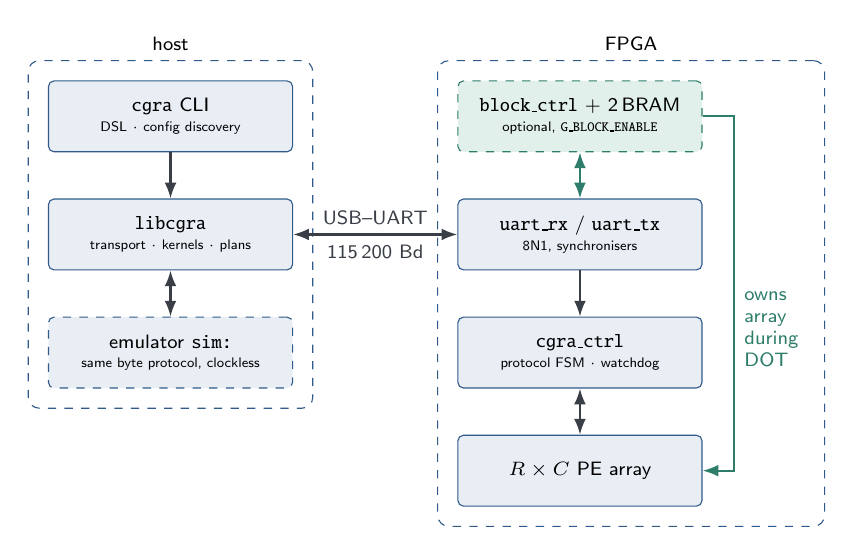
\begin{tikzpicture}[x=1mm, y=1mm, font=\scriptsize]
  \tikzset{b/.style={blk, minimum width=31mm, minimum height=9mm, font=\scriptsize}}
  % host
  \node[b] (cli) at (0,15) {\texttt{cgra} CLI\\[-0.3ex]{\tiny DSL $\cdot$ config discovery}};
  \node[b] (lib) at (0,0)  {\texttt{libcgra}\\[-0.3ex]{\tiny transport $\cdot$ kernels $\cdot$ plans}};
  \node[b, dashed] (emu) at (0,-15) {emulator \texttt{sim:}\\[-0.3ex]{\tiny same byte protocol, clockless}};
  \draw[wire] (cli) -- (lib);
  \draw[wireb] (lib) -- (emu);
  \begin{scope}[on background layer]
    \node[draw=cBlockE, dashed, rounded corners, fit=(cli)(emu), inner sep=2.5mm,
          label={[font=\scriptsize]above:host}] {};
  \end{scope}
  % fpga
  \node[b] (uart) at (52,0) {\texttt{uart\_rx} / \texttt{uart\_tx}\\[-0.3ex]{\tiny 8N1, synchronisers}};
  \node[b] (ctrl) at (52,-15) {\texttt{cgra\_ctrl}\\[-0.3ex]{\tiny protocol FSM $\cdot$ watchdog}};
  \node[b] (arr)  at (52,-30) {$R\times C$ PE array};
  \node[b, draw=cRegE, fill=cReg, dashed] (blk) at (52,15)
    {\texttt{block\_ctrl} + 2\,BRAM\\[-0.3ex]{\tiny optional, \texttt{G\_BLOCK\_ENABLE}}};
  \draw[wire] (uart) -- (ctrl);
  \draw[wireb] (ctrl) -- (arr);
  \draw[wireb, cRegE] (uart) -- (blk);
  \coordinate (own) at ($(blk.east)+(4,0)$);
  \draw[wire, cRegE] (blk.east) -- (own) |- node[lbl, pos=0.3, right, align=left, text=cRegE]
    {owns\\array\\during\\DOT} (arr.east);
  \coordinate (ownlbl) at ($(own)+(9,0)$);
  \begin{scope}[on background layer]
    \node[draw=cBlockE, dashed, rounded corners, fit=(blk)(arr)(ownlbl), inner sep=2.5mm,
          label={[font=\scriptsize]above:FPGA}] {};
  \end{scope}
  \draw[wireb] (lib) -- node[lbl, above] {USB--UART} node[lbl, below] {115\,200 Bd} (uart);
\end{tikzpicture}
}
  \caption{Host/device architecture. The command-line tool compiles a
  declarative configuration language into per-PE words and drives the library,
  which reaches either the FPGA over a USB--UART bridge or the clockless
  emulator speaking the same byte protocol. The block controller (dashed,
  green) exists only when the extension is elaborated.}
  \label{fig:stack}
\end{figure}


\section{Additional views of reported data}

Fig.~\ref{fig:timing} illustrates the capture spacing that the multicycle
argument of Section~P-\ref{P-sec:chain} relies on, for $D=3$ after a fused
reset. Figs.~\ref{fig:geometry} and~\ref{fig:sup-cost} plot data that the
paper reports in Table~P-\ref{P-tab:vivado} and Table~P-\ref{P-tab:measured}.
Fig.~\ref{fig:scaling} shows an earlier, separately archived sweep of
repeated dot products ($n=16$--1024, $r=1$--64, both vectors reused), whose
counts agree with the closed forms checked by its own script; the paper's
Fig.~P-\ref{P-fig:reuse} supersedes it by separating batching from reuse.

\begin{figure}[t]
  \centering
  % Registered step is high BEFORE the PE capture edge. D=3 is illustrated.
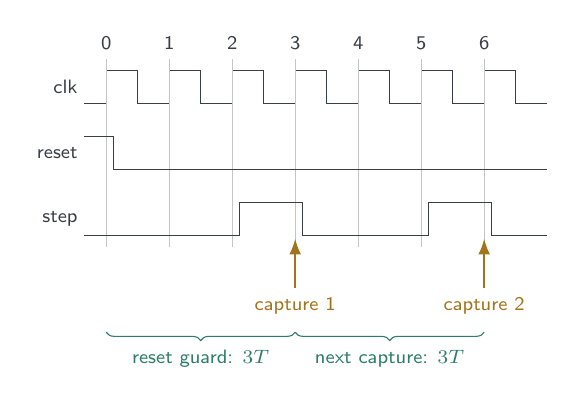
\begin{tikzpicture}[x=8mm, y=7mm, font=\scriptsize]
  \node[lbl, anchor=east] at (-0.3,3.3) {clk};
  \node[lbl, anchor=east] at (-0.3,2.1) {reset};
  \node[lbl, anchor=east] at (-0.3,0.9) {step};
  \draw[cWire] (-0.35,3) -- (0,3);
  \foreach \e in {0,...,6} {
    \draw[cWire] (\e,3) -- (\e,3.6) -- (\e+0.5,3.6) -- (\e+0.5,3) -- (\e+1,3);
    \draw[cWire!30] (\e,3.8) -- (\e,0.4);
    \node[lbl, above] at (\e,3.8) {\e};
  }
  % Control registers change just after the clock edge (offset for visibility).
  \draw[cWire] (-0.35,2.4) -- (0.12,2.4) -- (0.12,1.8) -- (7,1.8);
  \draw[cWire] (-0.35,0.6) -- (2.12,0.6) -- (2.12,1.2) -- (3.12,1.2)
    -- (3.12,0.6) -- (5.12,0.6) -- (5.12,1.2) -- (6.12,1.2)
    -- (6.12,0.6) -- (7,0.6);
  \foreach \e in {3,6} {
    \draw[wire,cAluE] (\e,-0.35) -- (\e,0.55);
  }
  \node[lbl, below, cAluE] at (3,-0.35) {capture 1};
  \node[lbl, below, cAluE] at (6,-0.35) {capture 2};
  \draw[decorate, decoration={brace,amplitude=3pt,mirror},cRegE]
    (0,-1.15) -- (3,-1.15);
  \draw[decorate, decoration={brace,amplitude=3pt,mirror},cRegE]
    (3,-1.15) -- (6,-1.15);
  \node[lbl,below,cRegE] at (1.5,-1.3) {reset guard: $3T$};
  \node[lbl,below,cRegE] at (4.5,-1.3) {next capture: $3T$};
\end{tikzpicture}

  \caption{Example with $D=3$ after EXEC reset. Reset changes the PE registers
  at edge 0; the first step captures at edge 3, then at edge 6. Stable source
  registers and the initial guard are required as well as periodic spacing.}
  \label{fig:timing}
\end{figure}


\begin{figure}[t]
  \centering
  \resizebox{\columnwidth}{!}{% figures/geometry — setup slack and register count of the five-shape sweep.
% Values are copied from verification/2026-10-05/geometry-physical/README.md
% (one routed run per shape); tables/geometry/table.tex lists the same data.
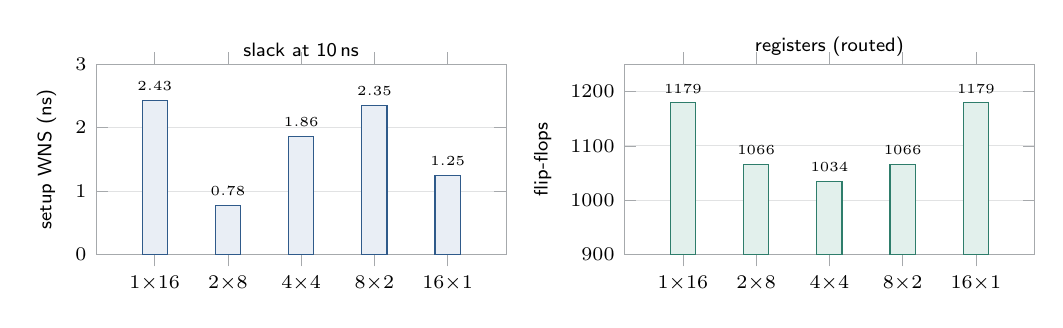
\begin{tikzpicture}
  \begin{axis}[
    name=wns, ybar, width=0.56\columnwidth, height=40mm, bar width=3.2mm,
    ymin=0, ymax=3, ytick={0,1,2,3}, ylabel={setup WNS (ns)},
    symbolic x coords={1x16,2x8,4x4,8x2,16x1}, xtick=data,
    xticklabels={$1{\times}16$,$2{\times}8$,$4{\times}4$,$8{\times}2$,$16{\times}1$},
    tick label style={font=\scriptsize}, label style={font=\scriptsize},
    axis line style={cWire!45}, tick style={cWire!45},
    ymajorgrids, grid style={cWire!15}, enlarge x limits=0.2,
    nodes near coords, every node near coord/.append style={font=\tiny},
    title={\scriptsize slack at 10\,ns}, title style={yshift=-1.5ex},
  ]
    \addplot[draw=cBlockE, fill=cBlock] coordinates
      {(1x16,2.433) (2x8,0.775) (4x4,1.862) (8x2,2.350) (16x1,1.247)};
  \end{axis}
  \begin{axis}[
    at={(wns.east)}, anchor=west, xshift=15mm,
    ybar, width=0.56\columnwidth, height=40mm, bar width=3.2mm,
    ymin=900, ymax=1250, ylabel={flip-flops}, ytick={900,1000,1100,1200},
    yticklabel style={/pgf/number format/1000 sep={}},
    every node near coord/.append style={/pgf/number format/1000 sep={}},
    symbolic x coords={1x16,2x8,4x4,8x2,16x1}, xtick=data,
    xticklabels={$1{\times}16$,$2{\times}8$,$4{\times}4$,$8{\times}2$,$16{\times}1$},
    tick label style={font=\scriptsize}, label style={font=\scriptsize},
    axis line style={cWire!45}, tick style={cWire!45},
    ymajorgrids, grid style={cWire!15}, enlarge x limits=0.2,
    nodes near coords, every node near coord/.append style={font=\tiny},
    title={\scriptsize registers (routed)}, title style={yshift=-1.5ex},
  ]
    \addplot[draw=cRegE, fill=cReg] coordinates
      {(1x16,1179) (2x8,1066) (4x4,1034) (8x2,1066) (16x1,1179)};
  \end{axis}
\end{tikzpicture}
}
  \caption{Five 16-PE geometries implemented from identical sources. All
  meet the 10\,ns constraint (positive slack, left). Register count follows
  the edge length $R+C$ (right; axis truncated at 900). Each point is one
  placement, so slack differences include placer variation.}
  \label{fig:geometry}
\end{figure}


\begin{figure}[t]
  \centering
  % Both this chart and the results table are rendered from data/wire-cost.csv.
\begin{tikzpicture}
  \begin{axis}[
    xbar, width=0.86\columnwidth, height=48mm, bar width=2.2mm,
    enlarge y limits=0.16, xmin=0, xmax=1.2,
    xtick={0,0.25,0.5,0.75,1}, xlabel={current v3 / current v2},
    symbolic y coords={vector,dot,scan,matvec,conv}, ytick=data,
    tick label style={font=\scriptsize}, label style={font=\scriptsize},
    axis line style={cWire!45}, tick style={cWire!45},
    xmajorgrids, grid style={cWire!18},
    extra x ticks={1}, extra x tick labels={},
    extra x tick style={grid=major,grid style={dashed,cWire!65}},
    legend style={at={(0.5,1.04)},anchor=south,legend columns=2,
      font=\scriptsize,draw=cWire!35},
  ]
    \addplot[draw=cBlockE,fill=cBlock] table[x=transactions,y=workload,col sep=comma]
      {build/wire-ratios.csv};
    \addlegendentry{transactions}
    \addplot[draw=cAluE,fill=cAlu] table[x=bytes,y=workload,col sep=comma]
      {build/wire-ratios.csv};
    \addlegendentry{total bytes}
  \end{axis}
\end{tikzpicture}

  \caption{Ratios of v3 to v2 transactions and bytes for the workloads of
  Table~P-\ref{P-tab:measured}; values below one indicate a reduction. Counts,
  not times.}
  \label{fig:sup-cost}
\end{figure}

\begin{figure}[t]
  \centering
  \resizebox{\columnwidth}{!}{% Measured on the emulator (data/scaling.csv): public-API wire bytes.
\begin{tikzpicture}
  \tikzset{every axis/.append style={width=0.56\columnwidth, height=44mm,
    tick label style={font=\scriptsize}, label style={font=\scriptsize},
    title style={font=\scriptsize, yshift=-1ex},
    axis line style={cWire!45}, tick style={cWire!45},
    xmajorgrids, ymajorgrids, grid style={cWire!15},
    legend style={font=\tiny, draw=cWire!35, fill=white}}}
  \begin{loglogaxis}[name=rep, title={(a) $r$ repeated calls, $n=256$},
      xlabel={repeated calls $r$}, ylabel={total wire bytes}, log basis x=2,
      xtick={1,4,16,64}, xticklabels={1,4,16,64},
      xmin=0.8, xmax=80, ymin=500, ymax=1e6,
      legend style={at={(0.03,0.97)}, anchor=north west}]
    \addplot[cAluE, mark=o, thick] table[x=repeat, y=v2, col sep=comma] {build/scaling-repeat.csv};
    \addlegendentry{v2}
    \addplot[cBlockE, mark=square*, mark size=1.4pt, thick] table[x=repeat, y=v3, col sep=comma] {build/scaling-repeat.csv};
    \addlegendentry{v3}
    \addplot[cRegE, mark=*, mark size=1.4pt, thick] table[x=repeat, y=blocks, col sep=comma] {build/scaling-repeat.csv};
    \addlegendentry{resident}
  \end{loglogaxis}
  \begin{loglogaxis}[at={(rep.east)}, anchor=west, xshift=12mm,
      title={(b) bytes per call versus $n$}, log basis x=2,
      xtick={16,64,256,1024}, xticklabels={16,64,256,1024},
      xlabel={vector length $n$}, ylabel={bytes per call},
      xmin=10, xmax=1500, ymin=40, ymax=5e4,
      legend style={at={(0.03,0.97)}, anchor=north west}]
    \addplot[cBlockE, mark=square*, mark size=1.4pt, thick] table[x=n, y=v3r1, col sep=comma] {build/scaling-length.csv};
    \addlegendentry{v3}
    \addplot[cRegE, mark=*, mark size=1.4pt, thick] table[x=n, y=blocksr1, col sep=comma] {build/scaling-length.csv};
    \addlegendentry{resident, $r=1$}
    \addplot[cRegE, mark=*, mark options={fill=white}, mark size=1.4pt, thick, densely dashed]
      table[x=n, y=blocksr64, col sep=comma] {build/scaling-length.csv};
    \addlegendentry{resident, $r=64$}
  \end{loglogaxis}
\end{tikzpicture}
}
  \caption{Repeated dot products through the public API, $4\times4$
  emulator, every result checked against a scalar reference. (a)~Legacy
  traffic grows linearly with the number of calls $r$; resident traffic is
  dominated by the one-time upload. (b)~Per-call bytes; for $r=64$ the
  upload is amortised. Counts, not times.}
  \label{fig:scaling}
\end{figure}


\section{Planned board acceptance}
\label{sec:board-plan}

No board was available. The acceptance procedure is fixed in advance, so
that a later run tests stated criteria rather than criteria chosen after the
fact.
\begin{enumerate}
  \item \emph{Artifact.} Program only a bitstream whose run manifest passes
        \texttt{make check-artifact}.
  \item \emph{Link.} \texttt{cgra probe} must receive an identification
        reply whose version and geometry equal the elaborated generics, then
        pass its known-answer tests.
  \item \emph{Function.} The kernels of the paper must reproduce the scalar
        references on the board for both protocol versions and the resident
        path.
  \item \emph{Timing.} Measure per-byte time and per-transaction turnaround
        $\tau$ on the actual USB--UART bridge with warm-up and repeated runs,
        report distributions, state the warm-up, repetition and outlier
        policy~\cite{hoefler-benchmarking}, and compare with a timed CPU
        baseline.
  \item \emph{Recovery.} Interrupt transfers, assert reset and let the
        watchdog expire; the host must report the session as uncertain and
        recover only through the documented reset path.
\end{enumerate}
Fig.~\ref{fig:board} shows the intended report. Its measured panels are
empty: they are generated from \texttt{doc/data/board/}, which holds only
column headers, and are marked NOT RUN. Panel~(b) already shows the model of
Eq.~P-\ref{P-eq:time} for $\tau=0$ and $\tau=16$\,ms for later comparison.
No synthetic data are shown as measurements.

\begin{figure*}[t]
  \centering
  \resizebox{\textwidth}{!}{% Board measurements (data/board/*.csv via tools/board_data.py). With empty
% CSV files every panel renders as a labelled NOT RUN placeholder.
\begin{tikzpicture}
  \node[anchor=north west, inner sep=0] (a) at (0,0) {\input{build/board-turnaround}};
  \node[anchor=north west, inner sep=0] (b) at ([xshift=4mm]a.north east) {\input{build/board-calls}};
  \node[anchor=north west, inner sep=0] (c) at ([xshift=4mm]b.north east) {\input{build/board-throughput}};
  \foreach \n/\t in {a/{(a) turnaround $\tau$}, b/{(b) time per call}, c/{(c) throughput}}
    \node[font=\scriptsize, anchor=south] at (\n.north) {\t};
\end{tikzpicture}
}
  \caption{Report format for board measurements: (a)~empirical
  distribution of $\tau$; (b)~measured call time against the model
  (solid: $\tau=0$; dashed: $\tau=16$\,ms); (c)~throughput against a timed CPU
  baseline. All measured series are NOT RUN.}
  \label{fig:board}
\end{figure*}

\section{Chronology of formal and implementation runs}

Every run below is archived with its inputs, commands, tool versions, logs
and source hashes; failed and inconclusive runs are kept as such.

\emph{Implementation.} An initial synthesis and STA run on 23 September
2026 concerned an earlier design and is superseded. On 5 October a complete
bitstream flow for the legacy $4\times4$ design passed all nine gates
(WNS $+1.862$\,ns, WHS $+0.098$\,ns) and five 16-PE shapes were implemented
from identical sources. The first period search failed its final gate,
because the requested period (5.859375\,ns) differed from the period applied
by the tool (5.859\,ns); after quantising periods to 1\,ps and checking the
applied clock, a second search on 6 October produced the 5.859\,ns
candidate. These runs used a top-level wrapper that predates the block
extension. On 7 October the enabled block build first failed to elaborate (a
boolean generic), then failed routed setup at $-3.580$\,ns and, after adding
operand registers, at $-2.867$\,ns on a path from state decoding into the
array multiplexers; an explicit ownership register with a proved guard led
to the passing run of 8 October (WNS $+0.427$\,ns). The synthesis pair of
Table~P-\ref{P-tab:block-cost} was produced the same day. For this paper the
legacy $4\times4$ design was re-implemented on the current revision at
10\,ns, reproducing the 5 October metrics exactly, and at 5.859\,ns
(\VivadoFastSummary).

\emph{Formal.} A monolithic $2\times3$ array proof timed out at 90\,s and a
first hierarchical PE formulation at 120\,s; the array is therefore proved
by composition with the separately proved PE transition. On 8 October the
full suite then in place reported 27 PROVED tasks and 8 required failures.
On 9 October an extended suite with the block properties reported 37
PROVED, 10 required failures and one UNKNOWN (block controller, $D=4$),
where induction did not close at the chosen depth; a separate run PROVED
that task after a reachable-state invariant was added as an assertion.
Several cover attempts for the block controller timed out or hit frontend
errors before the transcript driver was used. For this paper the complete
full and cover suites were re-executed on the current sources: 38 PROVED
tasks, all 10 negative and mutation tasks failing as required, no UNKNOWN,
and 18 reached covers. Only this last execution is reported as the formal
result of the paper.


\bibliographystyle{IEEEtran}
\bibliography{bib/bib}
\end{document}
